%%%%% this line is 80 chars wide, please don't make longer lines %%%%%%%%%%%%%%%
The "Auditory Neuroscience" book \cite{AuditoryNeuroscience} tells us in the 
chapter two what is important for us here to know. 

The peripheral auditory system has (generally air) pressure as input, 
and spike trains as output. We will go through the parts of the ear, with help 
of \autoref{fig:ear}. 

Let us consider first the external ear. There the pressure signals come through
 the ear canal and make the eardrum vibrate. 
This takes us to the medium ear. 
The vibration is propagated throughout it by three ossicles : malleus, incus 
and stapes. The farthest part from the external ear of the stapes touches the 
boundary of the cochlea, on the oval window, in the inner ear, 
and makes vibrate the liquid we find in it. 
The cochlea forms an interface between this mechanical vibration 
and the neural signal that will go through the auditory nerve 
(VII nerve on \autoref{fig:ear}).

%put that one page before the page it should appear on :
%http://www.andrewjpage.com/?archives/48-Figure-spanning-2-columns-in-Latex.html
\begin{figure*}[ht]
	\centering
  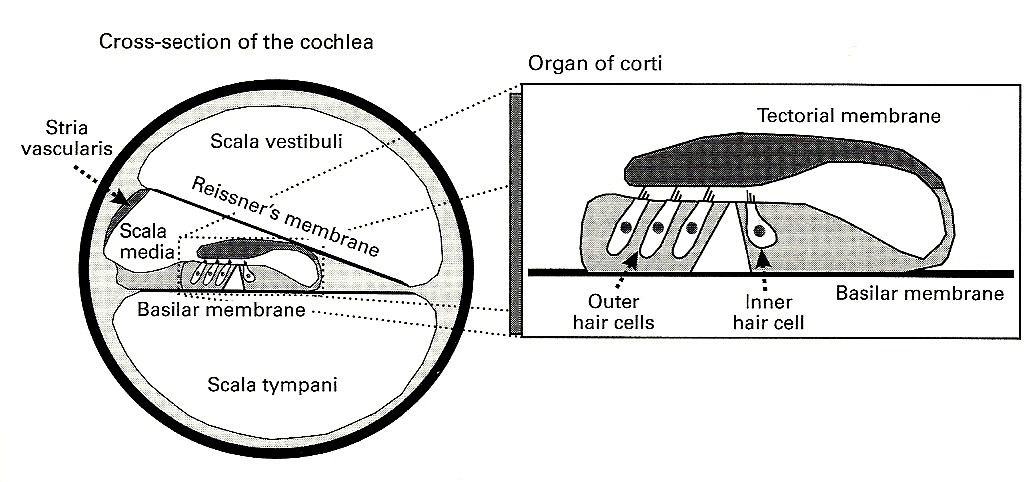
\includegraphics[width=0.75\textwidth]{images/corti2-aud65-level.jpg}
	\caption{Organ of Corti (\cite{AuditoryNeuroscience} p.65 )}
	\label{fig:corti}
\end{figure*}

%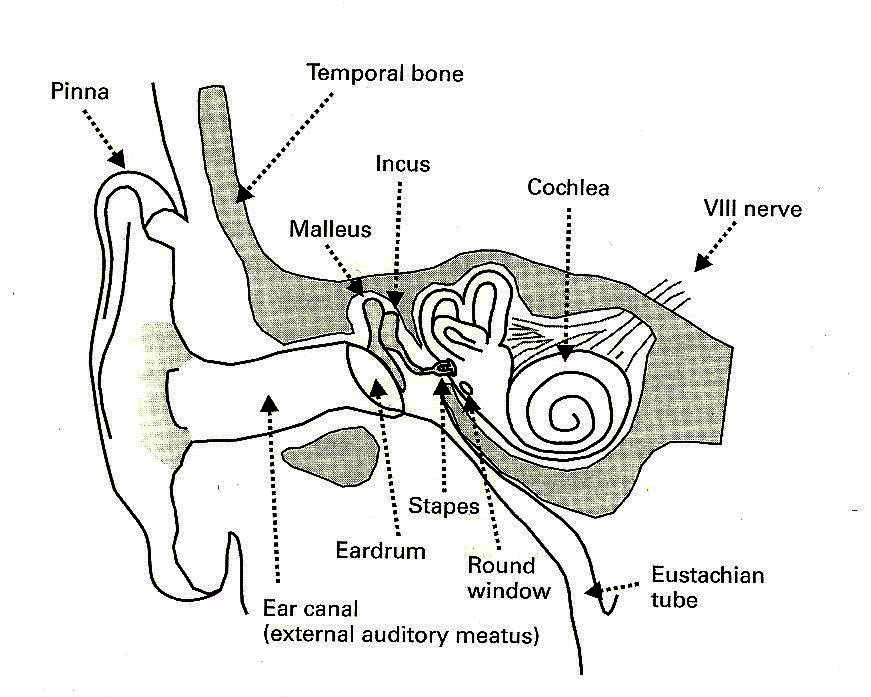
\includegraphics[width=0.45\textwidth]{images/ear-aud52-level.jpg}

\begin{figure}[h]
	\centering
	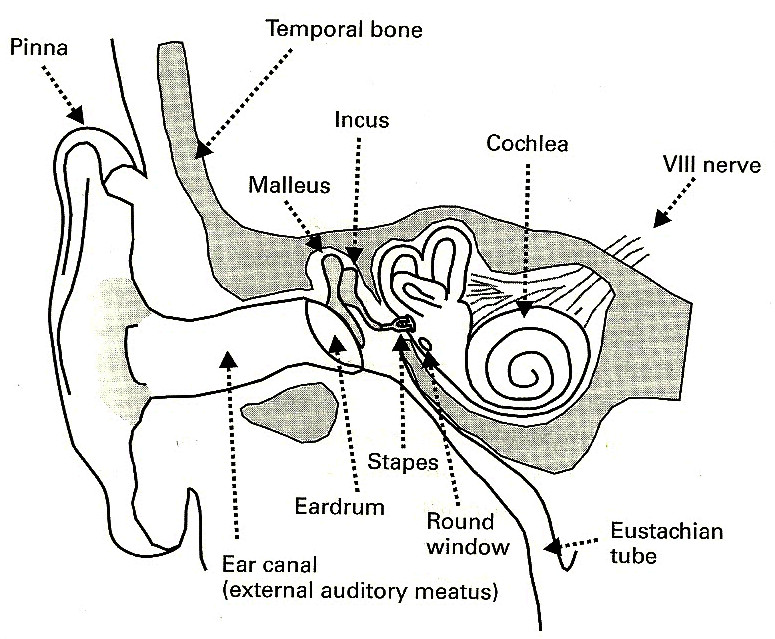
\includegraphics[width=0.45\textwidth]{images/ear2-aud52-level.jpg}
	\caption{Peripheral auditory system (\cite{AuditoryNeuroscience} p.52 )}
	\label{fig:ear}
\end{figure}

We will speak more about this interface below. But first we should see 
more about the vibration of the cochlea. 
The cochlea is a tube that has two main compartments which are placed on top of 
each other and separated throughout the cochlear tube by  
the basilar membrane,  except at the far end of it where they are joined, 
as you can see on \autoref{fig:ucochlea}.

%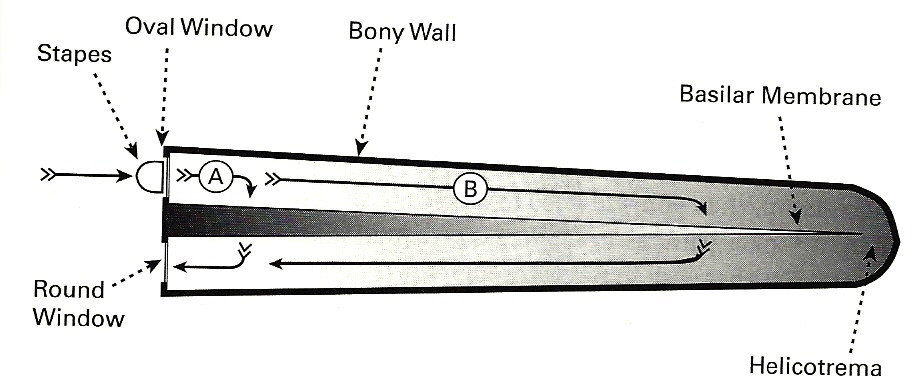
\includegraphics[width=0.45\textwidth]{images/cochlea-aud55-level.jpg}

\begin{figure}[h]
	\centering
	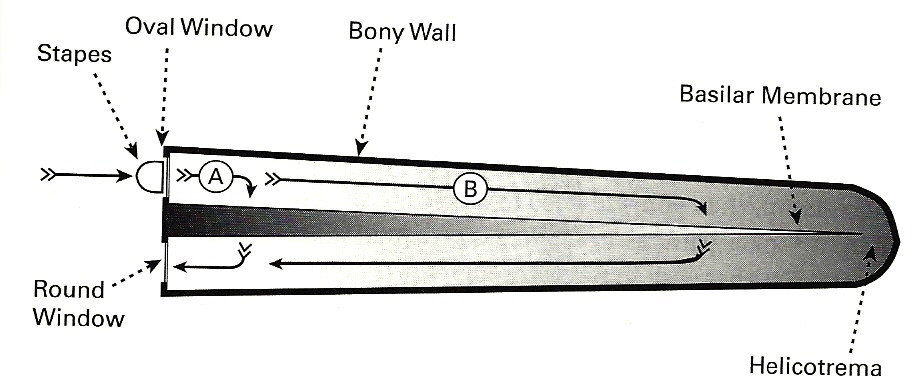
\includegraphics[width=0.45\textwidth]{images/cochlea-aud55-level.jpg}
	\caption{Unrolled cochlea (\cite{AuditoryNeuroscience} p.55 )}
	\label{fig:ucochlea}
\end{figure}


A vibration that comes will try to propagate through the basilar membrane from 
the upper compartment to the other. When doing that, it will not make all 
the parts of the basilar membrane vibrate at the same intensity. 
In fact, the cochlea is like a "biological Fourier analyzer" according to the book. 
The frequency content of vibrations is decomposed and each frequency has its 
"favorite" place in the cochlear coiled tube that it makes vibrate particularily. 
The part of the basilar membrane that is the first we can see vibrating, 
when we gradually put on the volume of a pure tone of frequency f, is said to be of 
"characteristic frequency" f. Near the oval window, the characteristic 
frequencies are high, and as we go to the tip of the tube, 
the characteristic frequency becomes lower.

Throughout the cochlear tube, we have the organ of Corti, which is the interface
about which an allusion was made above in the text. We will use \autoref{fig:corti} to illustrate our purpose.

%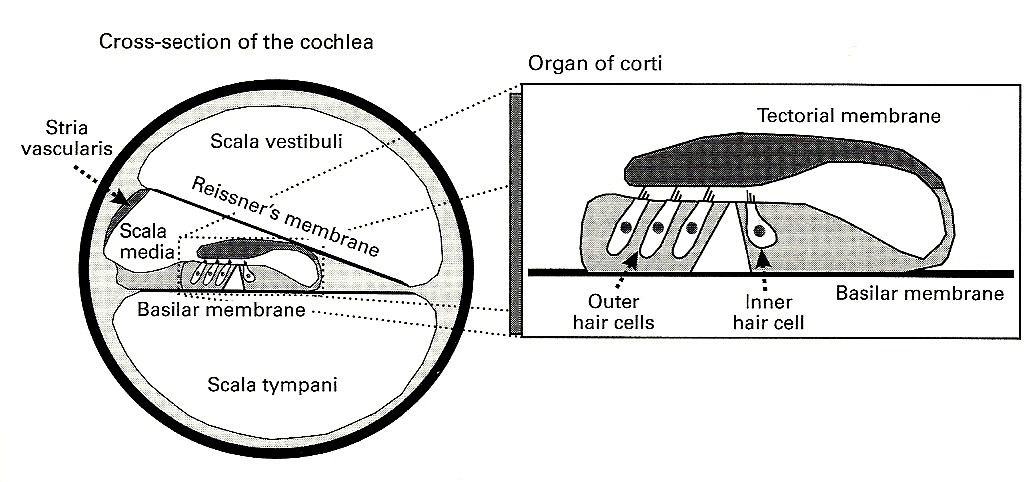
\includegraphics[width=0.45\textwidth]{images/corti2-aud65-level.jpg} %put before, so that then it is at right place

\begin{figure}[h]
	\centering
  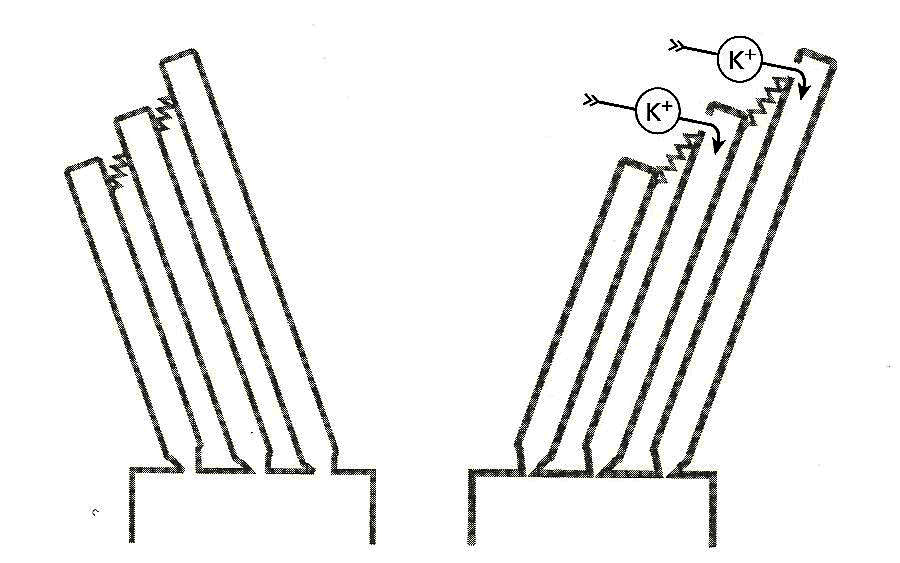
\includegraphics[width=0.45\textwidth]{images/hctransd-aud66-level.jpg}
	\caption{Transduction (\cite{AuditoryNeuroscience} p.66 )}
	\label{fig:transd}
\end{figure}

\begin{figure*}[ht]
	\centering
  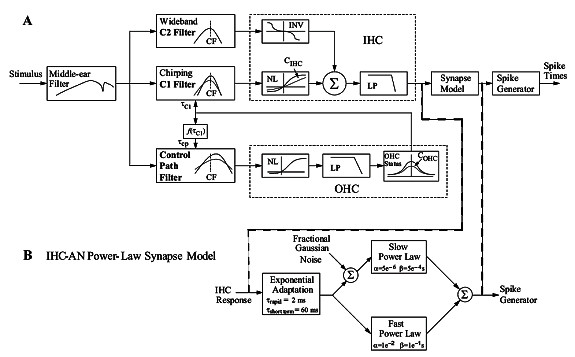
\includegraphics[width=0.75\textwidth]{images/www-bme-rochester-edu-schematicDiagram-level.jpg}
	\caption{Schema of the model (\cite{Model1} their fig. 2)}
	\label{fig:modelsch}
\end{figure*}

The upper compartment of the cochlea is in fact in two parts separated by a membrane.
The scala media, where we find the organ of Corti, has a higher 
concentration of potassium cations. We have as consequence a polarization between
the liquid of the scala media and the inner hair cells. 
When the basilar membrane vibrates, the tectorial membrane does 
that also and that makes the liquid move. 
These movements has as consequence the deflection of the stereocili 
of the inner hair cells, and when this happens, some potassium ions of the 
scala media go into the inner hair cells (IHC), and we have a depolarization.
%The outer hair cells undergo the same process, but , for their part, have a role of amplificator for the liquid movements. %% word about ohc ?
We can see that in \autoref{fig:transd}.
This has as consequence that some glutamate is leaked in synapses %glutamate checked : p75
between the IHC and the auditory nerve fibers, what excites these fibers 
and make them perhaps have some spikes.

%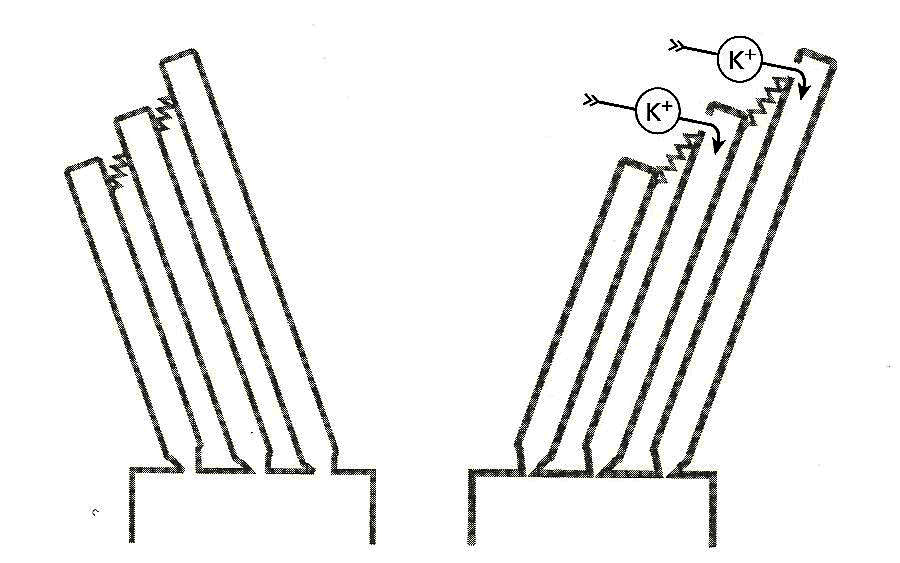
\includegraphics[width=0.45\textwidth]{images/hctransd-aud66-level.jpg}%put before, so that then it is at right place



